\clearpage
\twocolumn[{%
\rqparent
\subsection{Language transfer}
\label{app:rq06_language_transfer}

\noindent\begin{minipage}[t]{0.485\textwidth}
\vspace{0pt}
\paragraph{Research Question.} \emph{If a language's BPB is measured on only one or two small rungs, can the exponent pooled over the other languages predict its BPB at the reference size, also for languages the model never trained on? Does a design decision a proxy reads on its trained languages carry over to untrained ones? Which languages must a developer evaluate to recover the multilingual decision?}

\paragraph{Setup.} We test whether the language-list decision, read on a language's BPB, carries over to languages the lists do not train. We read the scheme A versus B decision at K $\in$ \{8, 15, 30\} on single-axis pairs, on the seed-1904 runs and sizes 90M--1.7B. The tasks are the per-language BPB of the 100 evaluation languages, grouped by whether both lists, one or neither trains them, and the untrained ones by whether a list trains their script. BPB has no chance level, so nothing is gated. DA-size compares the final checkpoint of each proxy (90M--1B) with that of the 1.7B run, and DA-ckpt the 1.7B run's checkpoints with its final one. Both are averaged over the three K. Per language family, we also measure how often tasks in untrained languages clear chance, against the English-only cell on the same tasks (Figure~\ref{fig:app_rq06_family_transfer}).
\end{minipage}\hfill
\begin{minipage}[t]{0.485\textwidth}
\vspace{0pt}
\begin{rqfinding}
\textbf{1. The list decision does not transfer to untrained languages at a proxy's scale.} Languages whose script a list trains are read at 0.63 at 90M and at 0.72--0.73 at 175M--600M, and reach 0.81 only at 1B. Languages in unseen scripts are read at 0.42--0.73 and never reach 0.75. By contrast, the languages that the lists train are read at 0.77--1.00 (both lists) and 1.00 (one list). (Figure~\ref{fig:app_rq06_language_transfer}.)
\\
\\
\textbf{2. Within one benchmark, the languages that a mixture trains together predict each other.} On HellaSwag (all languages), German, Spanish, French and Italian, the four European languages of the K8 list, predict each other's 1.7B ranking at 0.81 on average (Figure~\ref{fig:app_rq06_cross_task_hellaswag}), almost as well as each predicts itself (0.82).
\\
\\
\textbf{3. English is a poor proxy for the other languages.} English HellaSwag ranks itself at 0.78 but the other languages at only 0.43 on average, and they rank it at 0.50.
\end{rqfinding}
\end{minipage}

\vspace{\baselineskip}
\noindent\begin{minipage}{\textwidth}
\centering
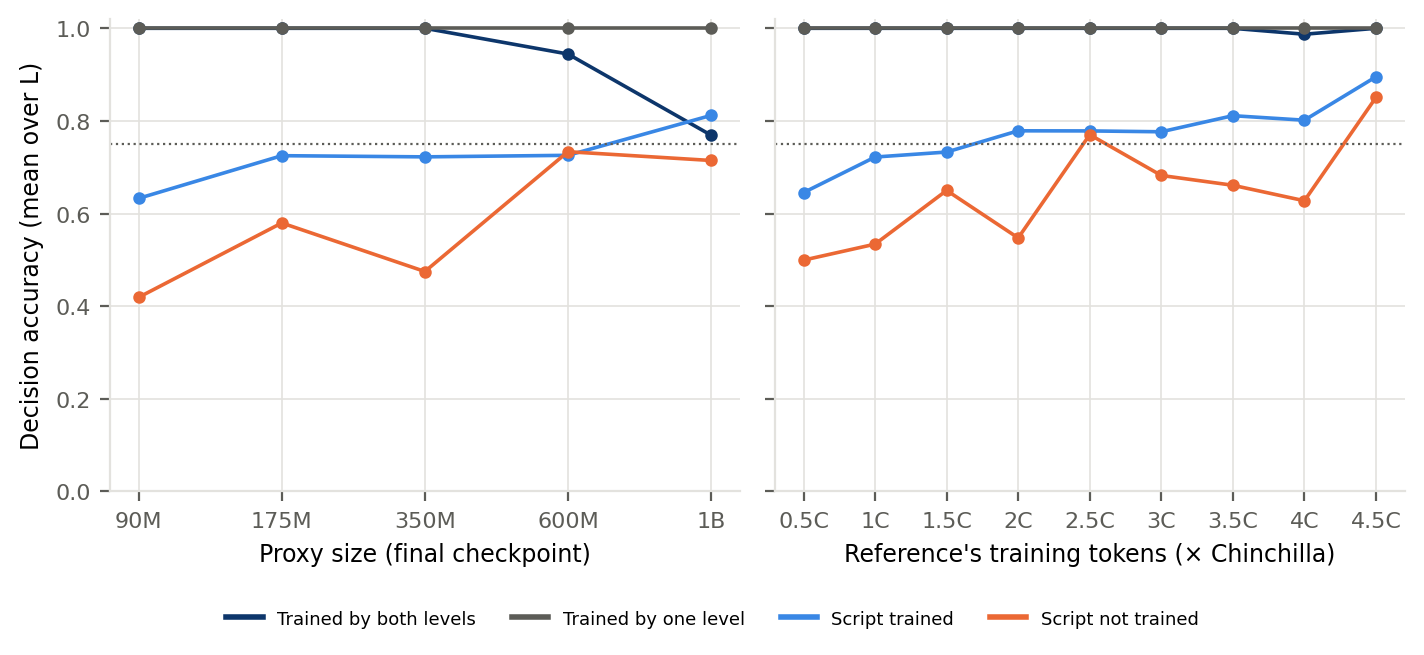
\includegraphics[width=\textwidth,height=0.36\textheight,keepaspectratio]{figures/app_rq06_language_transfer.png}
% source: src/signal-and-noise/analysis/rq06_language_transfer/pretraining/predictivity_seeds/transfer_da_all_lines_mono_axis_paper.png
\captionof{figure}{\textbf{The list decision does not transfer to untrained languages at a proxy's scale.} Decision accuracy (mean over K) of the language-list decision (scheme A vs B), read on the bits per byte of four groups of languages: trained by both lists, trained by one list, not trained but written in a trained script, and not trained in an untrained script. Left: DA-size by proxy size. Right: DA-ckpt along the 1.7B run, in Chinchilla multiples. The dotted line marks 0.75.}
\label{fig:app_rq06_language_transfer}
\end{minipage}
}]

\begin{figure*}[p]
\centering
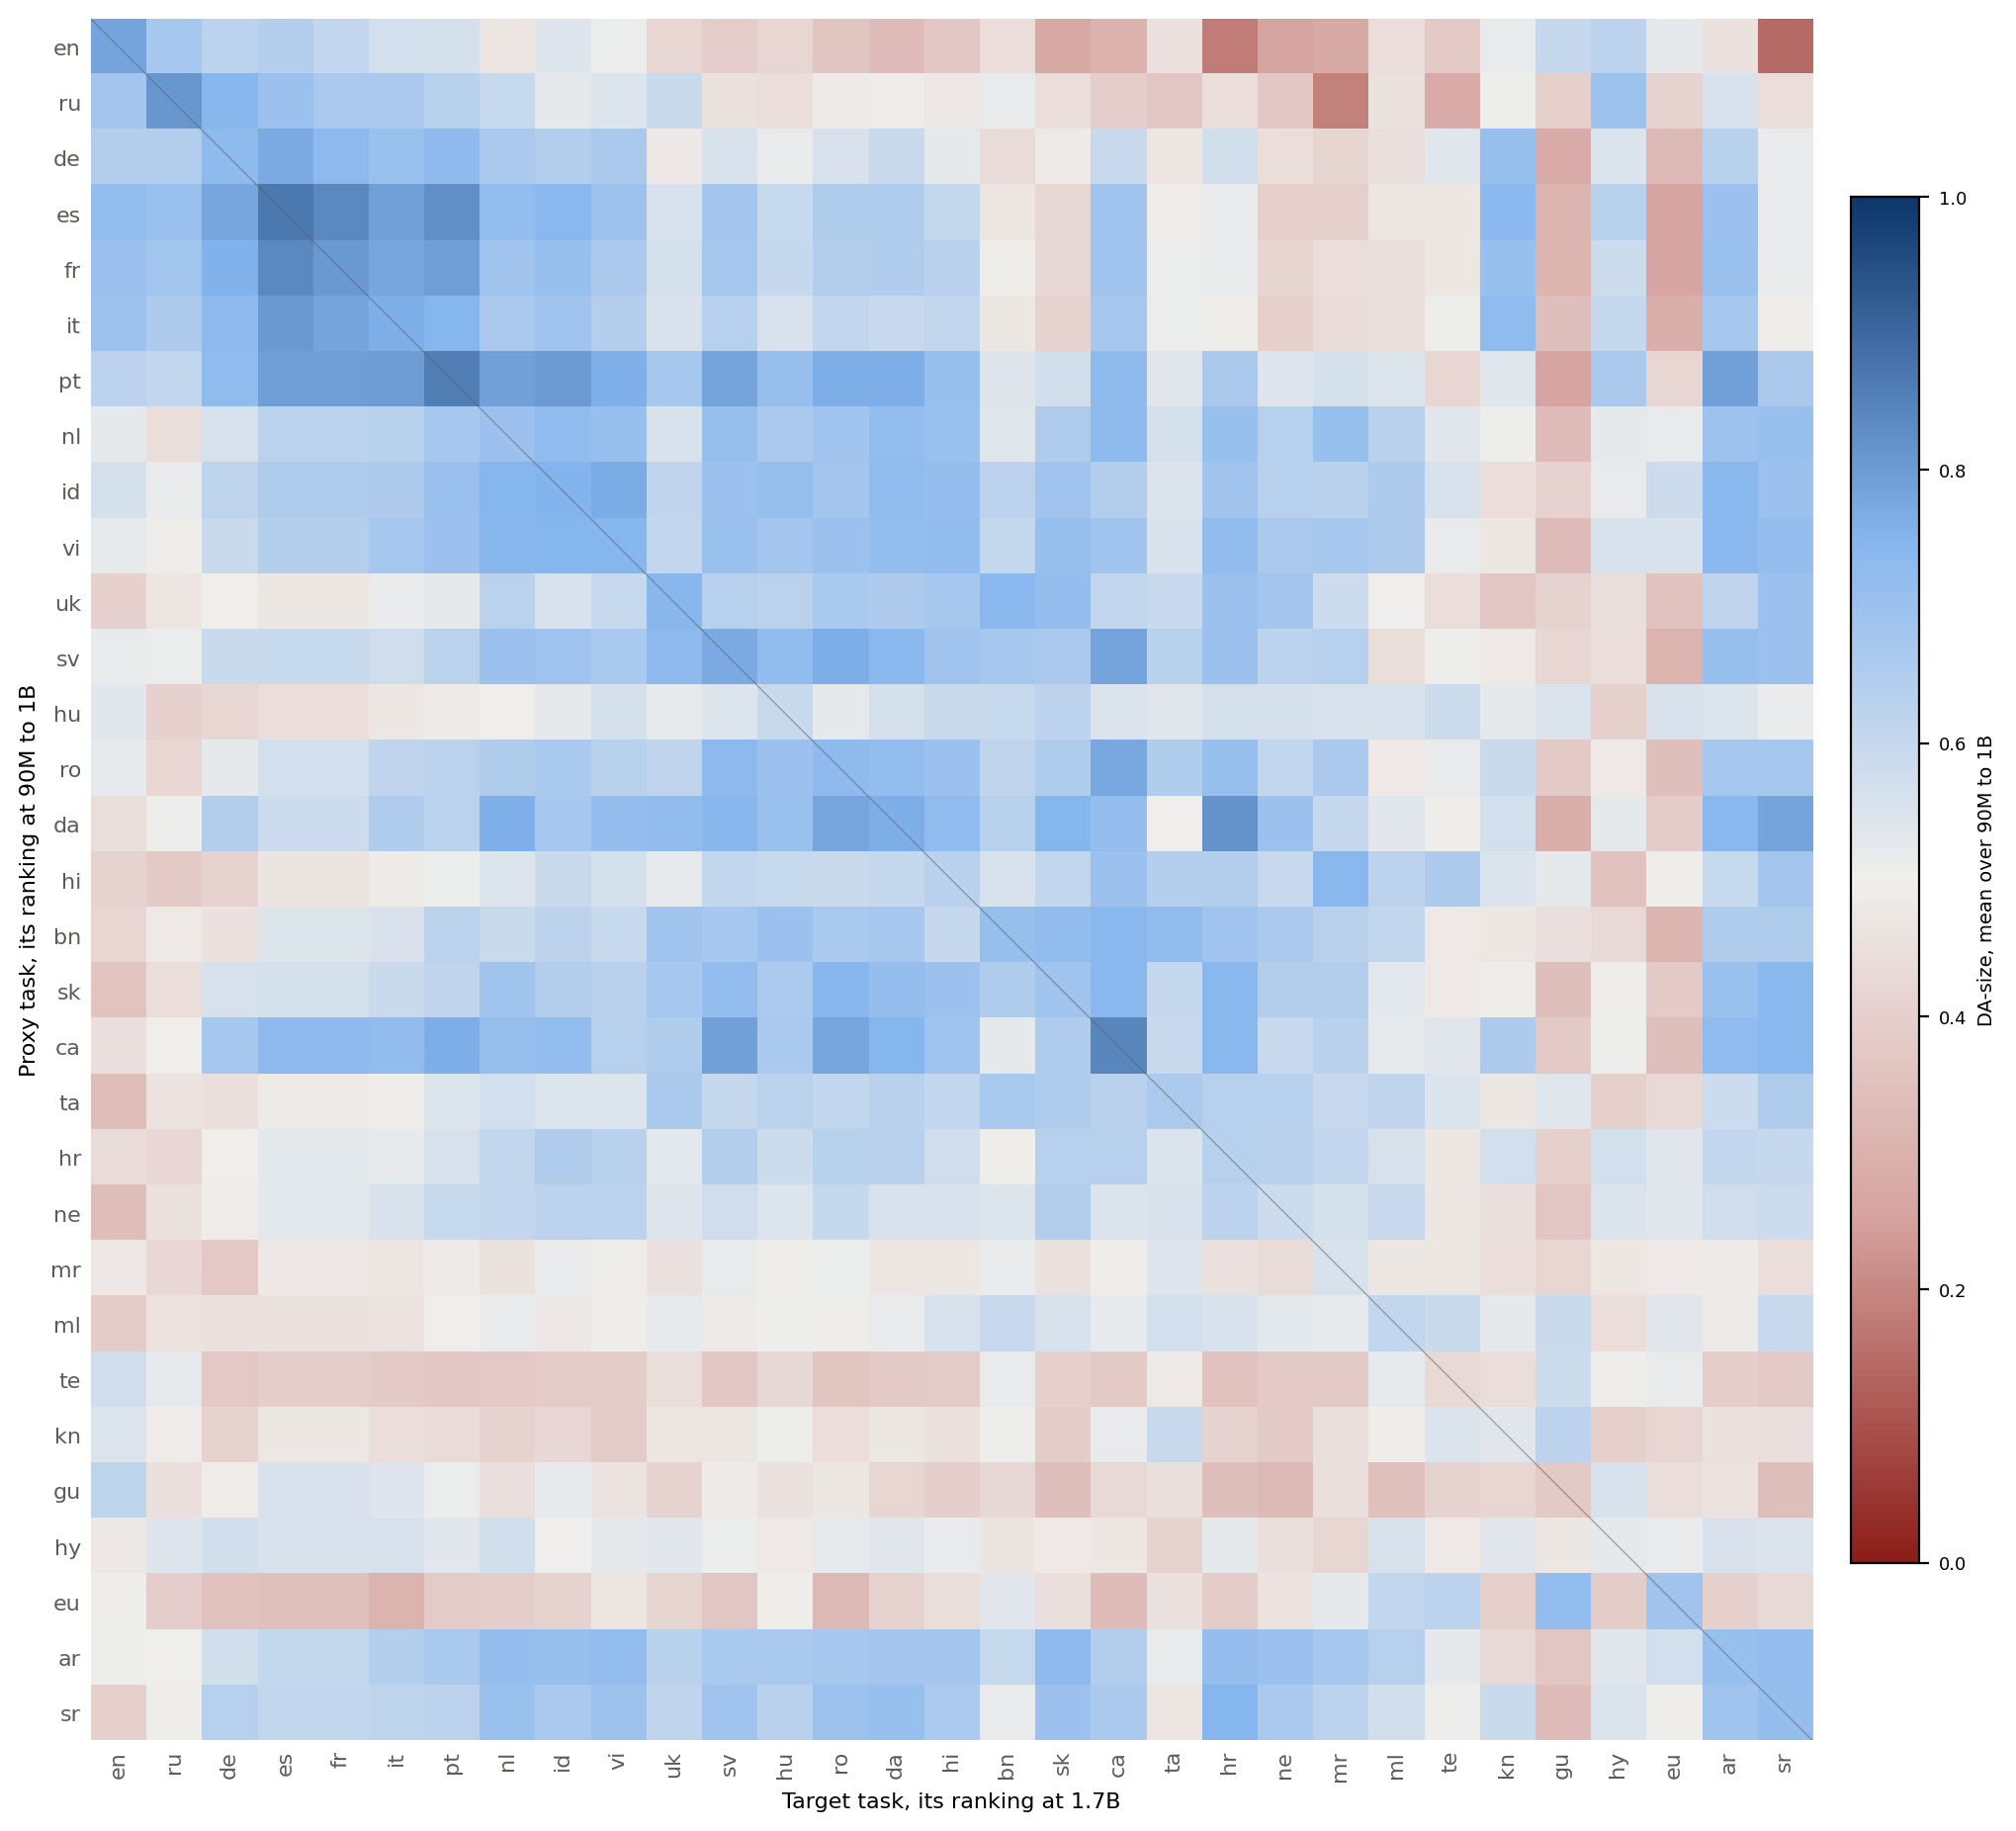
\includegraphics[width=0.8\textwidth,height=0.8\textheight,keepaspectratio]{figures/app_rq06_cross_task_hellaswag.png}
% source: src/signal-and-noise/analysis/rq06_language_transfer/pretraining/predictivity/cross_task_da_size_by_language_hellaswag_all_languages_mono_axis_paper.png
\caption{\textbf{On HellaSwag, German, Spanish, French and Italian, which the $K$ = 8 list trains together, predict each other's 1.7B ranking at 0.78, as well as each predicts its own (0.79), while English ranks the other languages at 0.45.} Each cell is the DA-size of the ranking of the design variants on the HellaSwag task of one language at a proxy size (rows) against the ranking on the task of another language at the 1.7B final checkpoint (columns), averaged over the proxies 90M--1B. The diagonal is the task's own DA-size. The pairs are the mono-axis design pairs of the seed-1904 runs, at least three per size, each task gated above chance at the size it is read at. A model's score on a language it does not train counts here. The scheme-A runs are evaluated on every language, so a language that no list trains, such as Basque (its column averages 0.44), is read on those runs alone. A cell averages the pairs both tasks have, so two cells may average different decisions. The colour is centred at 0.5, the agreement expected by chance. Languages follow the resource order of the training lists.}
\label{fig:app_rq06_cross_task_hellaswag}
\end{figure*}

\begin{figure*}[p]
\centering
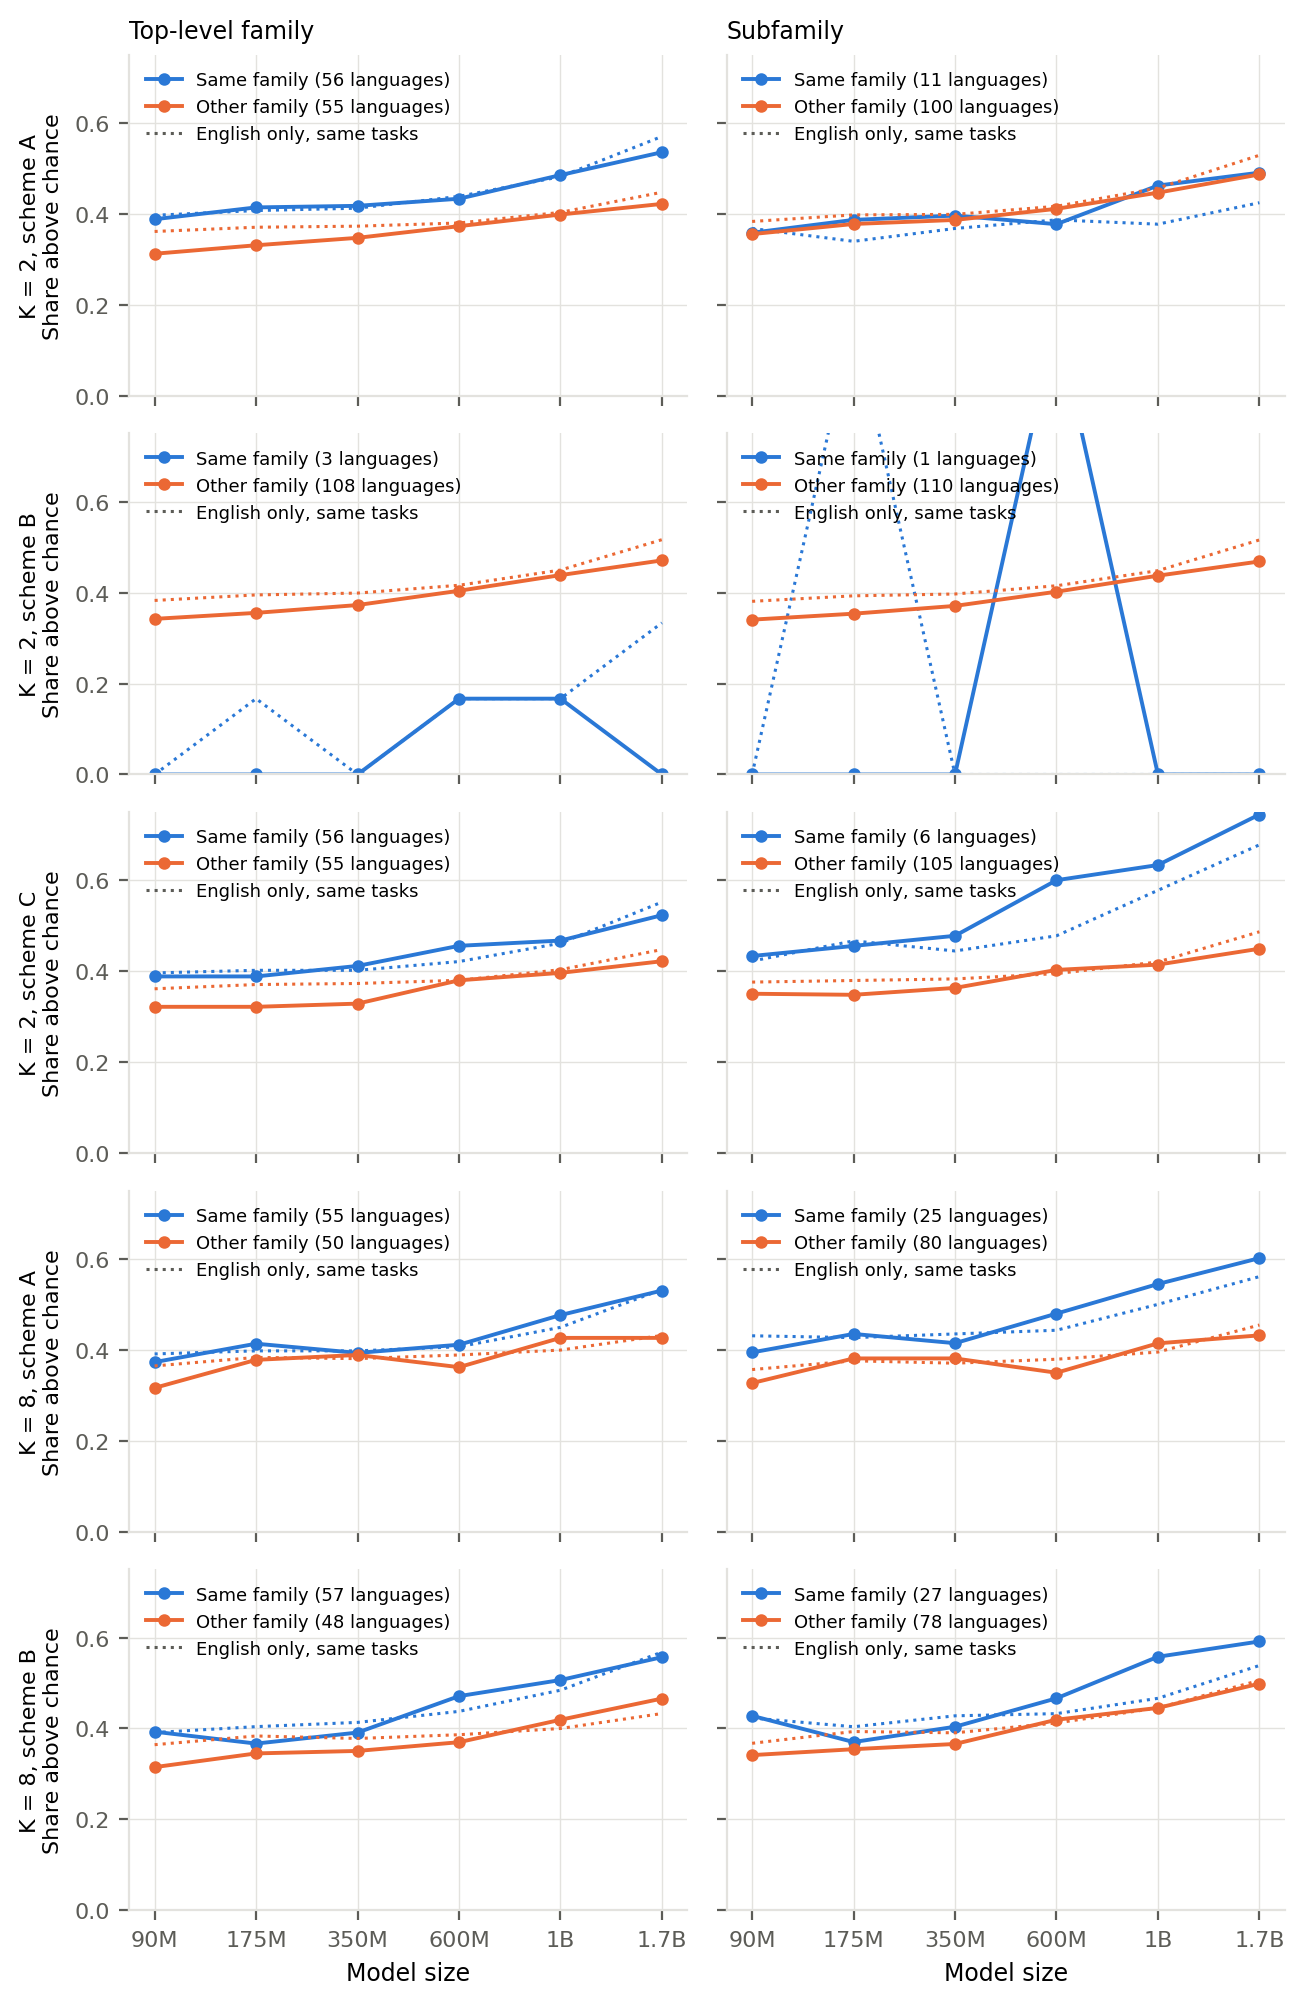
\includegraphics[width=\textwidth,height=0.8\textheight,keepaspectratio]{figures/app_rq06_family_transfer.png}
% source: src/signal-and-noise/analysis/rq06_language_transfer/pretraining/predictivity/above_chance_untrained_by_family_paper.png
\caption{\textbf{The $K$ = 8 scheme-A cell clears chance on more of its untrained same-subfamily tasks than the English-only cell does on the same tasks, by up to +0.04 at 1B, and on the other subfamilies by no more than +0.02.} Each panel is one cell (rows) and one family level (columns). A line is the share of the cell's accuracy tasks in untrained languages whose final run clears chance (on the benchmarks every cell is evaluated on, not on the candidates still being screened), split by whether the language shares the family of a trained non-English language (left: the top-level family such as Indo-European, right: the subfamily such as Slavic, from a Glottolog-style classification of every evaluated language). The dotted lines are the English-only $K$ = 1 cell on exactly the same tasks, so the gap between a solid line and its dotted twin is what training the cell's languages adds. Deep runs at seed 1904. Untrained languages are evaluated for the $K$ = 2 scheme-A cell at every size, the $K$ = 2 scheme-B cell at every size, the $K$ = 2 scheme-C cell at every size, the $K$ = 8 scheme-A cell at every size and the $K$ = 8 scheme-B cell at every size, some of them on part of the tasks so far. The $K$ = 1 cell has no 350M evaluation, so its dotted lines break there. Chinese has no subfamily of its own in the classification, so the $K$ = 2 scheme-B cell has no same-subfamily line.}
\label{fig:app_rq06_family_transfer}
\end{figure*}

